\documentclass[a4paper,10pt,twocolumn]{article}
\usepackage[utf8]{inputenc}
\usepackage[center]{caption}
\usepackage{subcaption}
\usepackage{bm}

% \usepackage[top=3cm, bottom=3cm, left=2cm, right=2cm]{geometry}

%---------------------------------------------
% MATLAB CODE PACKAGE
%---------------------------------------------
\usepackage{listings} 
\usepackage[usenames,dvipsnames]{color} % This is the color used for MATLAB comments below 
\definecolor{MyDarkGreen}{rgb}{0.0,0.4,0.0}
\lstset{
language=Matlab, % Use MATLAB 
frame=single, % Single frame around code 
basicstyle=\small\ttfamily, % Use small true type font 
keywordstyle=[1]\color{Blue}\bf, % MATLAB functions bold and blue 
keywordstyle=[2]\color{Purple}, % MATLAB function arguments purple 
keywordstyle=[3]\color{Blue}\underbar, % User functions underlined and blue identifier
style=, % Nothing special about identifiers % Comments small dark green courier 
commentstyle=\usefont{T1}{pcr}{m}{sl}\color{MyDarkGreen}\small, stringstyle=\color{Purple}, % Strings are purple
showstringspaces=false, % Don't put marks in string spaces 
tabsize=5, % 5 spaces per tab 
}
%---------------------------------------------
% Font packages
%---------------------------------------------
% \usepackage{lmodern}
% \usepackage{concmath}
% \usepackage{cmbright}
% \usepackage{kpfonts}
% \usepackage[adobe-utopia]{mathdesign}
\usepackage{fouriernc}
\usepackage[T1]{fontenc}

%---------------------------------------------
% Math environment packages & command
%---------------------------------------------
\usepackage{amsmath}
\usepackage{amssymb}
\usepackage{array}
\usepackage{mathrsfs}
\usepackage{array}
\def\sgn{\mathop{\rm sgn}\nolimits} 

\usepackage{schemabloc}


%---------------------------------------------
% item option
%---------------------------------------------
\renewcommand{\labelitemi}{-}


%---------------------------------------------
%HEADER & FOOTER
%---------------------------------------------
\usepackage{fancyhdr}
\pagestyle{fancy}

\renewcommand{\headrulewidth}{.15pt}
\fancyhead[C]{{Homework Assignment 2}} 
\fancyhead[L]{Page \thepage \ of \pageref{LastPage}}
\fancyhead[R]{MF2007}

\renewcommand{\footrulewidth}{.15pt}
\fancyfoot[C]{\thepage} 
% \fancyfoot[L]{truc}
% \fancyfoot[R]{\leftmark}

\usepackage{lastpage}

%---------------------------------------------
% two column option
%---------------------------------------------
\setlength{\columnsep}{1cm}

%---------------------------------------------
% Table of content
%---------------------------------------------
\usepackage[colorlinks,linkcolor=black, citecolor=black]{hyperref}

%opening
\title{MF2007: Dynamic \& Motion Control \\ Workshop 2}
\author{Kilian \textsc{Demeulemeester}, Jeremy \textsc{Pouech} \\ \texttt{\{kiliande,pouech\}@kth.se}}

\begin{document}

\setlength\parindent{0em}

\maketitle

\tableofcontents

\begin{abstract}
 This paper summarizes our work on servo control, code implementation on a microprocessor and analysis of the robustness to parameter uncertainty and sensor noise. The first and second part use the result from workshop A about how to control a DC-motor in position, improving the controller by using a model following block and a trajectory planner. The last part deals with closed loop poles positionning in the case of a valved controlled hydraulic cylinder.
\end{abstract}
  

\part*{Servo Control} 
\addcontentsline{toc}{part}{Servo Control}

\section*{Model following control}
\addcontentsline{toc}{section}{Model following control}

\subsection*{Level 1}
\addcontentsline{toc}{subsection}{Level 1}


Here, we will design a model following controller by inverting the process model in the time domain.

The control structure is depicted in Figure \ref{contStruct}.

\begin{figure}[ht]
\begin{center}
$$\text{TO BE CREATED}$$
\end{center}
 \caption{Control structure for the DC-motor}
 \label{contStruct}
\end{figure}

The model following block is depicted in Figure \ref{modelFollow}.

\begin{figure}[ht]
\begin{center}
$$\text{TO BE CREATED}$$
\end{center}
 \caption{Model following for the DC-motor}
 \label{modelFollow}
\end{figure}

Since the DC-motor model we used is a second order system, the reference position must be two times differentiable. 

The trajectory planner is design using the fastest possible positionning:
\begin{equation}a_{max} = \frac{\pm M_{max}}{J}\end{equation}
\begin{equation}v_{max} = \frac{U_{max} - \frac{R}{k_\varphi} F_c}{\frac{R d}{k_\varphi} + k_\varphi}\end{equation}

With:

$M_{max}$ : maximum torque of the motor

$v_{max}$ : maximum reachable velocity of the DC-motor, computed with the DC motor model equations.





	
\clearpage

\part*{Writing Controller Code} 
\addcontentsline{toc}{part}{Writing controller code}

%------------------------------------------------
% 		LEVEL 1
%------------------------------------------------
\subsection*{Level 1}
\addcontentsline{toc}{subsection}{Level 1}

The embedded Matlab implementation leads to the exact same result than the implementation using ordinary Simulink blocks. Indeed, since we use a discretize controller, transposing the simulink code to the embedded Matlab implementation produce the a code with the same behavior as the one produced by Simulink.

Figure \ref{embedded} show the superposition of the embedded implementation and the one using Simulink.


\begin{figure}[ht]
  \centering
  \begin{subfigure}[b]{\linewidth}
   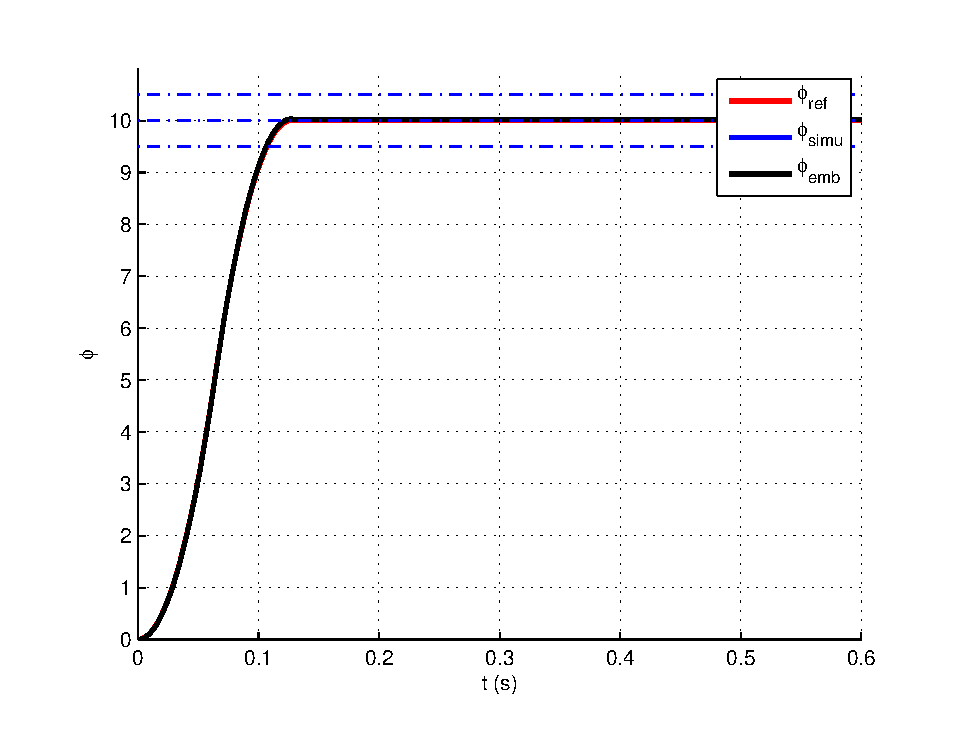
\includegraphics[width=\columnwidth]{fig/embeddedlvl110.eps}
   \caption{$Rs = 10$[rad]}
  \end{subfigure}
  \begin{subfigure}[b]{\linewidth}
  \includegraphics[width=\columnwidth]{fig/embeddedlvl1100.eps}
   \caption{$Rs = 100$[rad]}
  \end{subfigure}

 \caption{Result with a embedded controller}
 \label{embedded}
\end{figure}

%------------------------------------------------
% 		LEVEL 2
%------------------------------------------------
\subsection*{Level 2}
\addcontentsline{toc}{subsection}{Level 2}
	

\clearpage

\part*{Robustness to Parameter Uncertainty and Sensor Noise}
\addcontentsline{toc}{part}{Robustness}

This part aim to control a valve for a hydraulic cylinder. Figure \ref{valve} shows the non symetric vavle driven hydraulic cylinder. 

\begin{figure}
 \includegraphics[width=\linewidth]{fig/valve.ps}
 \caption{Valve controlled hydraulic cylinder}
 \label{valve}
\end{figure}

%------------------------------------------------
% 		LEVEL 2
%------------------------------------------------
\subsection*{Level 2}
\addcontentsline{toc}{subsection}{Level 2}

We want to design a velocity controler for the valve controlled hydraulic cylinder -- using a continuous controller. 

The system will be simulate using the following reference:
\begin{itemize}
 \item $r(t) = 0.5 \text{ m/s}$
 \item Zero external force
\end{itemize}

\subsubsection*{Real model}
The system is described by the following equations:

$$
\begin{array}{rcl}
    m \dot{v} & = & p_1 A_1 - p_2 A_2 - d v - f_e \\
    Q_{1v} & = & R_v \sqrt{p_s - p_1} x_v \\
    Q_{2v} & = & R_v \sqrt{p_2 - p_r} x_v \\
    Q_1 & = & Q_{1v} - Q_c \\
    Q_2 & = & - Q_{2v} + Q_c \\
    Q_c & = & A v \\
    C_f \dot{p_1} & = & Q_1 \\
    C_f \dot{p_2} & = & Q_2 \\
\end{array}
$$

With:

$p_i$: internal pression in area $i$

$m$: mass of piston

$A_i$: effective piston area

$f_e$: external force

$d$: friction coefficient

$Q_c$: volume flow due to piston velocity

$Q_{iv}$: flow from/out area $i$

$C_f$: fluid capacitance

$p_s, p_t$: supplied pression, tank pression

$R_v$: flow constant

\subsubsection*{Linear model}
We linearize the model around an operating point:

$$\begin{array}{rcl}
   x_v & = & x_{vQ} + \Delta x_v \\
   p_1 & = & p_{1Q} + \Delta p_1 \\
   p_2 & = & p_{2Q} + \Delta p_2 \\
  \end{array}$$

Let $$x = \left[\begin{array}{ccc}x_1 & x_2 & x_3 \end{array}\right]^T = \left[\begin{array}{ccc} \Delta v & \Delta p_1 & \Delta p_2 \end{array}\right]^T$$ and $$u = \left[\begin{array}{cc}u_1 & u_2 \end{array}\right]^T = \left[\begin{array}{cc} \Delta x_v & f_e \end{array}\right]^T$$

Then:

$$ \begin{array}{rcl} 
    \bm{A} & = & \left(\frac{\partial f_i}{\partial x_j}\right)_{i,j} \\
    \bm{B} & = & \left(\frac{\partial f_i}{\partial u_j}\right)_{i,j}
   \end{array}$$
   
Thus:

$$ \begin{array}{rcl}
    \dot{x} & = &  \bm{A}x + \bm{B}u \\
    y & = & \bm{C}x + \bm{D}u
   \end{array}$$
   
With:

$$\begin{array}{rcl}
   \bm{A} & = & \left(\begin{array}{ccc} 
   -\frac{d}{m} & \frac{A}{m} & -\frac{A}{m} \\ 
   -\frac{A}{C_f} & -\frac{1}{C_f} \frac{R_v x_{vQ}}{2\sqrt{p_s - p_{1Q}}} & 0 \\ 
   \frac{A}{C_f} & 0 & \frac{1}{C_f} \frac{-R_v x_{vQ}}{2 \sqrt{p_{2Q}-p_t}}
   \end{array}\right) \\ \\
   
   \bm{B} & = & \left(\begin{array}{cc}
   0 & \frac{1}{m} \\
   \frac{R_v \sqrt{p_s - p_{1Q}}}{C_f} & 0 \\
   \frac{-R_v \sqrt{p_s - p_{1Q}}}{C_f} & 0 \\
   \end{array}\right) \\ \\
   
   \bm{C} & = & \left(\begin{array}{ccc}
   1 & 0 & 0\\
   \end{array}\right) \\ \\
   
   \bm{D} & = & 0 \\
  \end{array}$$

\subsubsection*{Control design}

The matrix $\bm{A}$ and $\bm{B}$, using the numerical values, are:

$$\begin{array}{rcl}
   \bm{A} & \approx & 1e9 \left(\begin{array}{ccc} 
   0 & 0 & 0 \\ 
   -2.86 & 0 & 0 \\ 
   2.86 & 0 & 0
   \end{array}\right) \\ \\
   
   \bm{B} & \approx & 1e11 \left(\begin{array}{cc}
   0 & 0 \\
   5 & 0 \\
   5 & 0 \\
   \end{array}\right) \\ \\
  \end{array}$$
  
 \textbf{Remark:} Some values seems to be equal to zero, but are actually really small towards the other ones. Our Matlab implementation does not use zero.
 
 
 
 Thus, the close-loop transfert function is equal to:
 
 $$H(s) = \frac{B(s)}{A(s)} = \bm{C}(s\bm{I}-\bm{A})^{-1}\bm{B}$$

\clearpage

\appendix

\onecolumn

\section{Writing Controller Code}
\label{appendixCode}
   
\begin{lstlisting}
function [ac,vc,rc,u] = fcn(Rs,t)
%#codegen
%% Variable declarations

Ts = 1e-3;
amax = 3000;
vmax = 300;
d = 5.8e-6;
J = 1/2200000;
Fc = 1e-4;
R = 24;
kM = 8.64e-3;
kE = 30/pi*0.905e-3;

%% Trajectory computation
t1 = vmax/amax;
t2 = Rs/vmax;
t1p = sqrt(Rs/amax);

if t1 > t2
    t1 = t1p;
    t2 = t1p;
end

t3 = t1+t2;

ac = 0;
vc = 0;
rc = 0;
if t < t1
    ac = amax;
    vc = amax*t;
    rc = amax*t^2/2;
end
if t >= t1 && t < t2
    ac = 0;
    vc = amax*t1;
    rc = amax*t1^2/2 + amax*t1*(t-t1);
end
if t >= t2 && t < t3
    ac = -amax;
    vc = amax*t1 - amax*(t-t2);
    rc = amax*t1^2/2 + amax*t1*(t2-t1) +amax*t1*(t-t2) - amax*(t-t2)^2/2;
end
if t >= t3
    ac = 0;
    vc = 0;
    rc = Rs;
end

%% Feedforward loop
u = R*(J*ac + d*vc + sign(vc) * Fc)/kM + kE * vc;

\end{lstlisting}

\end{document}
